\chapter{The Single Top Quark Dataset}
\label{selectioncuts}
\label{analysis}
\label{data}

This chapter describes the dataset and analysis strategy used in the search for single top quark production. This analysis is a continuation of previous single top quark searches at $\dzero$ as summarized in Section~\ref{previous}. The dataset used in the latest analysis is divided into independent samples or channels in which the single top quark analysis is performed and later combined when measuring the cross section. The division of analysis channels and the general measurement strategy is described in Section~\ref{strategy}. The triggers used to select single top-like events at runtime are described in Section~\ref{datasample}. The integrated luminosity recorded for the dataset is also reported in this section. A set of selection cuts is applied to the data set to remove mis-measured events or events which are unlikely single top quark candidates. In general the cuts are designed to select events with one high $p_{T}$ lepton from the $W$ boson decay, large missing $E_{T}$ indicating a neutrino in the final state, and two to four jets. All selection cuts are explained in Section~\ref{objectselection} with a summary table of expected fraction of $s$-channel and $t$-channel remaining after the cuts have been applied.

\section{Previous Single Top Searches}
\label{previous}

There have been several searches for single top quark production by the $\dzero$ and CDF collaborations. During Run I $\dzero$ published two analyses~\cite{Abbott:2000pa, Abazov:2001ns} using $90$~pb$^{-1}$ and set limits of $\sigma_{s-\rm{channel}} < 17$~pb and $\sigma_{t-\rm{channel}} < 22$~pb both at 95$\%$ confidence level. The CDF collaboration also published two analyses~\cite{Acosta:2004er, Acosta:2001un} using $106$~pb$^{-1}$ of Run I data resulting in limits of  $\sigma_{s-\rm{channel}} < 18$~pb and $\sigma_{t-\rm{channel}} < 13$~pb at $95\%$ confidence level.

During Run II both $\dzero$ and CDF have performed several searches for single top. $\dzero$ has published two analyses~\cite{Abazov:2005zz,Abazov:2006uq} using $230$~pb$^{-1}$ and CDF has published one analysis~\cite{Acosta:2004bs}. Both $\dzero$ and CDF have released preliminary analyses using 370 pb$^{-1}$~\cite{run2-d0-370} and 700~pb$^{-1}$~\cite{run2-cdf-bnn-700}, respectively, with improved limits.  Table~\ref{previouslimits} summarizes the limits on both $s$-channel and $t$-channel single top quark production.

\vspace{0.2in}
\begin{table}[!h!tbp]
\begin{center}
\caption{Summary of limits on $s$-channel, $t$-channel, and combined $s+t$-channel single top quark production from the $\dzero$ and CDF collaborations.}
\label{previouslimits}
\begin{tabular}{c|ccc}
%\multicolumn{4}{c}{\underline{Upper Limits on Single Top Quark Production [pb]}} \vspace{0.1in} \\
%	Analysis							&	\multicolumn{3}{c}{Production Channel} \\
Analysis									&	$s$-channel & $t$-channel & Combined $s+t$ \\
\hline
Tevatron Run I							&		&		&		\\
\hline
~~~~~~~~~~$\dzero$ with 90~pb$^{-1}$		&	17	&	22	&	-	\\
~~~~~~~~~~CDF with 106~pb$^{-1}$		&	18	&	13	&	14	\\
\hline
Tevatron Run II							&		&		&		\\
\hline
~~~~~~~~~~$\dzero$ with 162~pb$^{-1}$	&	19	&	25	&	23	\\
~~~~~~~~~~CDF with 162~pb$^{-1}$		&	13.6	&	10.1	&	17.8	\\
~~~~~~~~~~$\dzero$ with 230~pb$^{-1}$	&	6.4	&	5.0	&	-	\\
~~~~~~~~~~~~~~~~~~~~~~$\dzero$ with 370~pb$^{-1}$ (prelim.)	&	5.0	&	4.4	&	-	\\
~~~~~~~~~~~~~~~~~~~~~~CDF with 700~pb$^{-1}$ (prelim.)		&	3.2	&	2.9	&	3.4	\\
\end{tabular}
\vspace{-0.1in}
\end{center}
\end{table}

The CDF collaboration recently released three analyses using $955$~pb$^{-1}$ of Run II data. One analysis~\cite{run2-cdf-me-955} measures the combined $s$-channel and $t$-channel cross section of $2.7^{+1.5}_{-1.3}$~pb with a 2.3$\sigma$ signal significance. The other two analyses~\cite{run2-cdf-nn-955,run2-cdf-lhood-955} do not observe a significant excess of data above background and set limits on the combined $s+t$-channel production of 2.6 and 2.7~pb$^{-1}$ at 95$\%$ confidence level.

\section{Analysis Measurement Strategy}
\label{strategy}

The single top quark measurement strategy is to divide the data into many orthogonal samples, perform the analysis in each sample, and combine them during the cross section extraction procedure. The data are divided by lepton flavor, the number of reconstructed jets, and by the number of $B$-tags. The division by lepton flavor is due to the trigger selection and because events with electrons and muons suffer from different types of backgrounds. The division by the number of reconstructed jets is to ensure proper background modeling by the Monte Carlo for each jet multiplicity. Finally, the division by the number of $B$-tags is due to different sensitivities to either $s$-channel or $t$-channel events. For instance, events with one $B$-tag are sensitive to both $s$-channel and $t$-channel single top while events with two $B$-tags are only sensitive to $s$-channel events. In total there are twelve independent channels corresponding to two lepton channels (electron and muon), three reconstructed jet channels (two, three, and four), and two $B$-jet channels (one and two tags).

\section{Triggers for Single Top Quark Events}
\label{datasample}

The Run II dataset used in the single top quark analysis was collected by the $\dzero$~detector between August 2002 and December 2005. During this time there have been eight distinct periods in which the triggers used to collect data events have changed. All triggers are described in the following two sections.

\subsection{Electron Channel Trigger}
Electron channel events are selected by triggering on events with at least one electron and at least two jets~\footnote{At the trigger level an electron is still considered a jet because it deposits energy in the calorimeter in a similar way to jets.}. The electron trigger used in the single top quark analysis has changed five times during the entire run period. A description of the five triggers used is given below. Table~\ref{electrontrigger} summarizes the triggers used to collect electron single top quark events and the total integrated luminosity recorded with each trigger.

\begin{itemize}
\item $\rm{EM15\_2JT15}$
\begin{itemize}
\item Level1: One EM calorimeter tower with $E_{T}>10$~GeV and two jet calorimeter towers with $E_{T}>5$~GeV.
\item Level2: One EM object with $E_{T}>10$~GeV and electromagnetic fraction $>$~0.85. Also two jet objects with $E_{T}>10$~GeV.
\item Level3: One EM object with $E_{T}>15$~GeV and a shower shape consistent an EM object. Also, two jet objects with $E_{T}>15$~GeV.
\end{itemize}
\item $\rm{E1\_SHT15\_2J20}$
\begin{itemize}
\item Level1: One EM calorimeter tower with $E_{T}>11$~GeV.
\item Level2: No requirement.
\item Level3: One EM object with $E_{T}>15$~GeV and a shower shape consistent an EM object. Also, two jet objects with $E_{T}>20$~GeV.
\end{itemize}
\item $\rm{E1\_SHT15\_2J\_J25}$
\begin{itemize}
\item Level1: One EM calorimeter tower with $E_{T}>11$~GeV.
\item Level1: One EM object with $E_{T}>15$~GeV.
\item Level2: No requirement.
\item Level3: One EM object with $E_{T}>15$~GeV and a shower shape consistent an EM object. Also, two jet objects with $E_{T}>20$~GeV. One of the jets is also required have $E_{T}>25$~GeV.
\end{itemize}
\item $\rm{E1\_SHT15\_2J\_J30}$
\begin{itemize}
\item Level1: One EM calorimeter tower with $E_{T}>11$~GeV.
\item Level1: One EM object with $E_{T}>15$~GeV.
\item Level2: No requirement.
\item Level3: One EM object with $E_{T}>15$~GeV and a shower shape consistent an EM object. Also, two jet objects with $E_{T}>20$~GeV. One of the jets is also required have $E_{T}>30$~GeV.
\end{itemize}
\end{itemize}

\vspace{0.2in}
\begin{table}[!h!tbp]
\begin{center}
\caption{Integrated luminosities by trigger version for the triggers used to record electron single top quark events. The total integrated luminosity is shown in bold.}
\label{electrontrigger}
\begin{tabular}{cc|c}
%\multicolumn{3}{c}{\underline{Electron Triggers}}\vspace{0.1in}\\
Trigger Period	&	Trigger Name		&	Integrated Luminosity [pb$^{-1}$]	\\
\hline
I	&	E1\_SHT15\_2J15		&	103 \\ 
II	&	E1\_SHT15\_2J20		&	227 \\ 
III	&	E1\_SHT15\_2J\_J25	&	55 \\
IV	&	E1\_SHT15\_2J\_J30	&	294 \\ 
V	&	E1\_SHT15\_2J\_J25	&	234 \\
\hline
\multicolumn{2}{c|}{Total Integrated Luminosity}
                                   &  {\bf 913} \\
\end{tabular}
\vspace{-0.1 in}
\end{center}
\end{table}


\subsection{Muon Channel Trigger}

Muon channel events are selected by triggering on events with at least one muon and at least one jet. The muon trigger used in the single top quark analysis has changed seven times during the entire run period. A description of the seven triggers used is given below. Table~\ref{muontrigger} summarizes the triggers used to collect muon single top quark events and the total integrated luminosity recorded with each trigger.

\begin{itemize}
\item $\rm{MU\_JT20\_L2M0}$
\begin{itemize}
\item Level1: One muon with scintillator and wire hit and one calorimeter tower with $E_{T}>5$~GeV.
\item Level2: One muon object.
\item Level3: One jet object with $E_{T}>20$~GeV.
\end{itemize}
\item $\rm{MU\_JT25\_L2M0}$
\begin{itemize}
\item Level1: One muon with scintillator and wire hit and one calorimeter tower with $E_{T}>5$~GeV.
\item Level2: One muon object.
\item Level3: One jet object with $E_{T}>25$~GeV.
\end{itemize}
\item $\rm{MUJ2\_JT25}$
\begin{itemize}
\item Level1: One muon with scintillator and wire hit and one calorimeter tower with $E_{T}>5$~GeV.
\item Level2: One muon object and a jet object with $E_{T}>8$~GeV.
\item Level3: One jet object with $E_{T}>25$~GeV.
\end{itemize}
\item $\rm{MUJ2\_JT25\_LM3}$
\begin{itemize}
\item Level1: One muon with scintillator and wire hit and one calorimeter tower with $E_{T}>5$~GeV.
\item Level2: One muon object and a jet object with $E_{T}>8$~GeV.
\item Level3: One jet object with $E_{T}>25$~GeV and a muon object with p$_{T}>3$~GeV.
\end{itemize}
\item $\rm{MUJ2\_JT30\_LM3}$
\begin{itemize}
\item Level1: One muon with scintillator and wire hit and one calorimeter tower with $E_{T}>5$~GeV.
\item Level2: One muon object and a jet object with $E_{T}>8$~GeV.
\item Level3: One jet object with $E_{T}>30$~GeV and a muon object with p$_{T}>3$~GeV.
\end{itemize}
\item $\rm{MUJ1\_JT25\_ILM3}$
\begin{itemize}
\item Level1: One muon with scintillator and wire hit and one calorimeter tower with $E_{T}>5$~GeV.
\item Level2: One muon object and a jet object with $E_{T}>8$~GeV.
\item Level3: One jet object with $E_{T}>25$~GeV and an isolated muon object with p$_{T}>3$~GeV.
\end{itemize}
\item $\rm{MUJ1\_JT35\_LM3}$
\begin{itemize}
\item Level1: One muon with scintillator and wire hit and one calorimeter tower with $E_{T}>5$~GeV.
\item Level2: One muon object and a jet object with $E_{T}>8$~GeV.
\item Level3: One jet object with $E_{T}>35$~GeV and a muon object with p$_{T}>3$~GeV.
\end{itemize}
\end{itemize}

\vspace{0.2in}
\begin{table}[!h!tbp]
\begin{center}
\caption{Integrated luminosities by trigger version for the triggers used to record muon single top quark events. The total integrated luminosity is shown in bold.}
\label{muontrigger}
\begin{tabular}{cc|c}
%\multicolumn{3}{c}{\underline{Muon Triggers}}\vspace{0.1in}\\
Trigger Period	&	Trigger Name		&	Integrated Luminosity [pb$^{-1}$]	\\
\hline
I	&	MU\_JT20\_L2M0		&	109 \\ 
II	&	MU\_JT25\_L2M0		&	231 \\ 
III	&	MUJ2\_JT25			&	31 \\
IV	&	MUJ2\_JT25\_LM3		&	16 \\
V	&	MUJ2\_JT30\_LM3		&	252 \\
VI	&	MUJ1\_JT25\_ILM3		&	21 \\
VII	&	MUJ1\_JT35\_LM3		&	214 \\
\hline
\multicolumn{2}{c|}{Total Integrated Luminosity}
                                   &  {\bf 871} \\
\end{tabular}
\vspace{-0.1 in}
\end{center}
\end{table}


\section{Reconstructed Object Selection}
\label{objectselection}

The following sections describe the selection cuts applied to the data. The goal of the selection cuts is to remove events which are unlikely single top candidates as well as remove events which may mimic the single top quark event signature, but are created by detector noise or low energy physics processes in the event.


\subsection{Lepton Selection}

Leptons in the event must be consistent with a $W$ decay thus are required to have \mbox{$p_{T}>15 (18)$~GeV} and $|\eta|<1.1(2.0)$ for electrons (muons). To remove $Z \rightarrow \ell \ell$+jets and $\dilepton$ events a veto on additional leptons with $p_{T}>15$~GeV is applied. Events with a high $p_{T}$ muon veto event with an electron and visa versa to ensure orthogonality between search channels. Fig.~\ref{stmuon} shows the expected muon $p_{T}$ and $\eta$ distribution for $s$-channel and $t$-channel single top.

\begin{figure}[!h!tbp]
\begin{center}
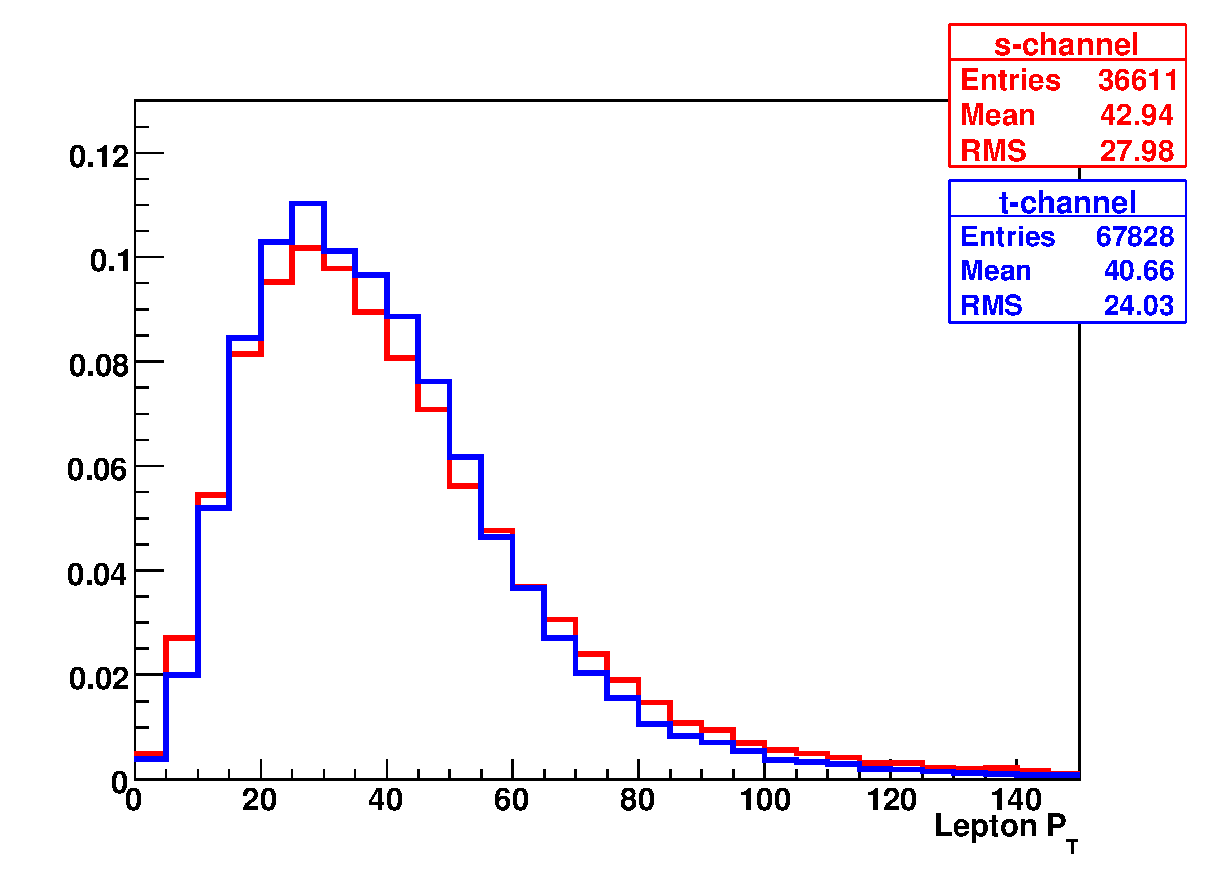
\includegraphics[width=0.48\textwidth]{eps/Analysis/LeptonPt.eps}
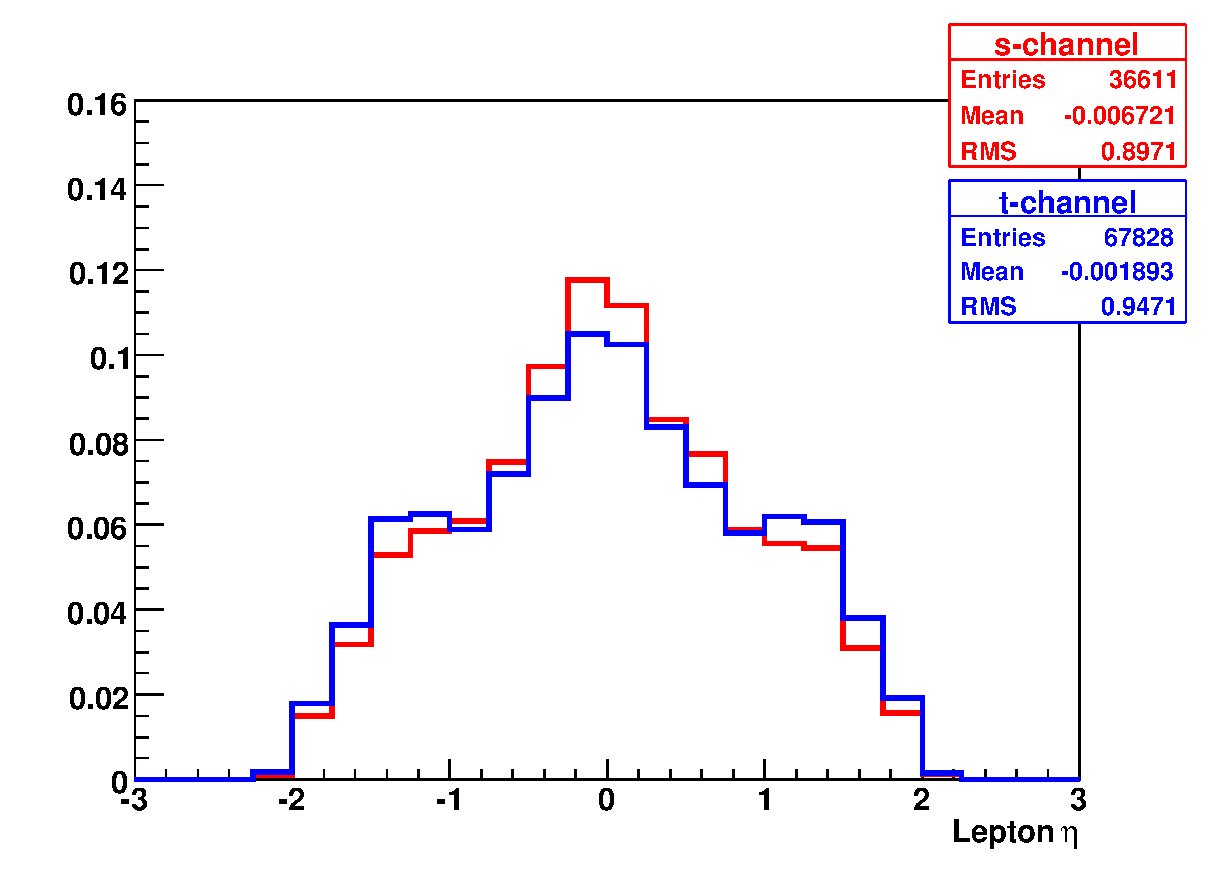
\includegraphics[width=0.48\textwidth]{eps/Analysis/LeptonEta.eps}
\end{center}
\vspace{-0.1in}
\caption{Muon $p_{T}$ (left) and $\eta$ (right) distributions for $s$-channel (red) and $t$-channel (blue) single top. Muons are required to have $p_{T}>18$~GeV and $|\eta|<2$.}
\label{stmuon}
\end{figure}

\subsection{Jet Selection}
\label{jetselection}

Leading order $s$-channel and $t$-channel single top quark events have at most three partons in the final state which will likely yield either two or three jets. To account for higher order radiation effects events are allowed to have between two and four fully corrected jets. The leading jet (highest $p_{T}$) must have $p_{T}>25$~GeV and $|\eta^{det}|<2.5$. The second jet (second highest $p_{T}$) must have $p_{T}>20$~GeV and $|\eta^{det}|<3.4$. All other jets in the event must have $p_{T}>15$~GeV and $|\eta^{det}|<3.4$. Fig.~\ref{stjet1} shows the expected leading $p_{T}$ and $\eta$ distribution for $s$-channel and $t$-channel single top and Fig.~\ref{stjet2} shows the same distributions for the second leading jet.

\begin{figure}[!h!tbp]
\begin{center}
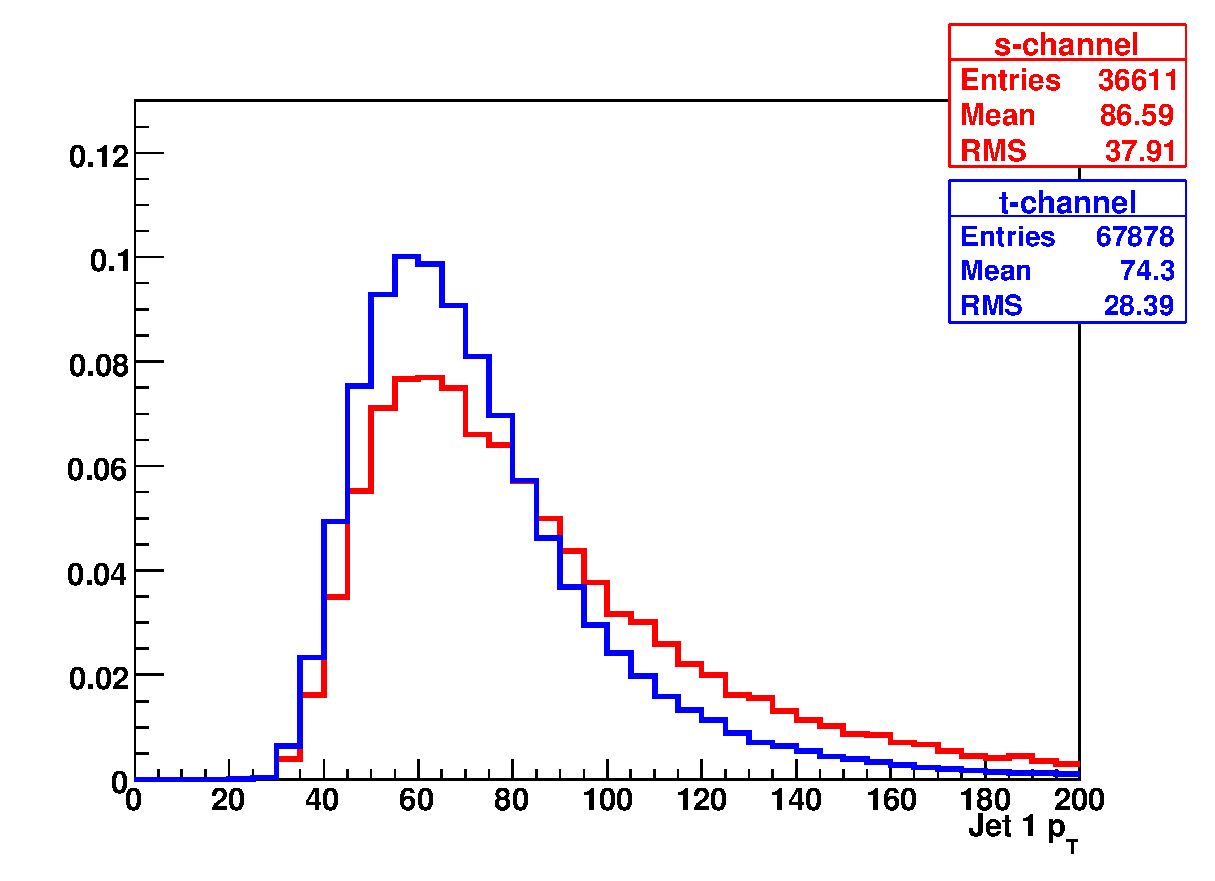
\includegraphics[width=0.48\textwidth]{eps/Analysis/Jet1Pt.eps}
\includegraphics[width=0.48\textwidth]{eps/Analysis/Jet1Eta.eps}
\end{center}
\vspace{-0.1in}
\caption{Leading jet $p_{T}$ (left) and $\eta$ (right) distributions for $s$-channel (red) and $t$-channel (blue) single top. The leading jet is required to have $p_{T}>25$~GeV and $|\eta|<2.5$}
\label{stjet1}
\end{figure}

\begin{figure}[!h!tbp]
\begin{center}
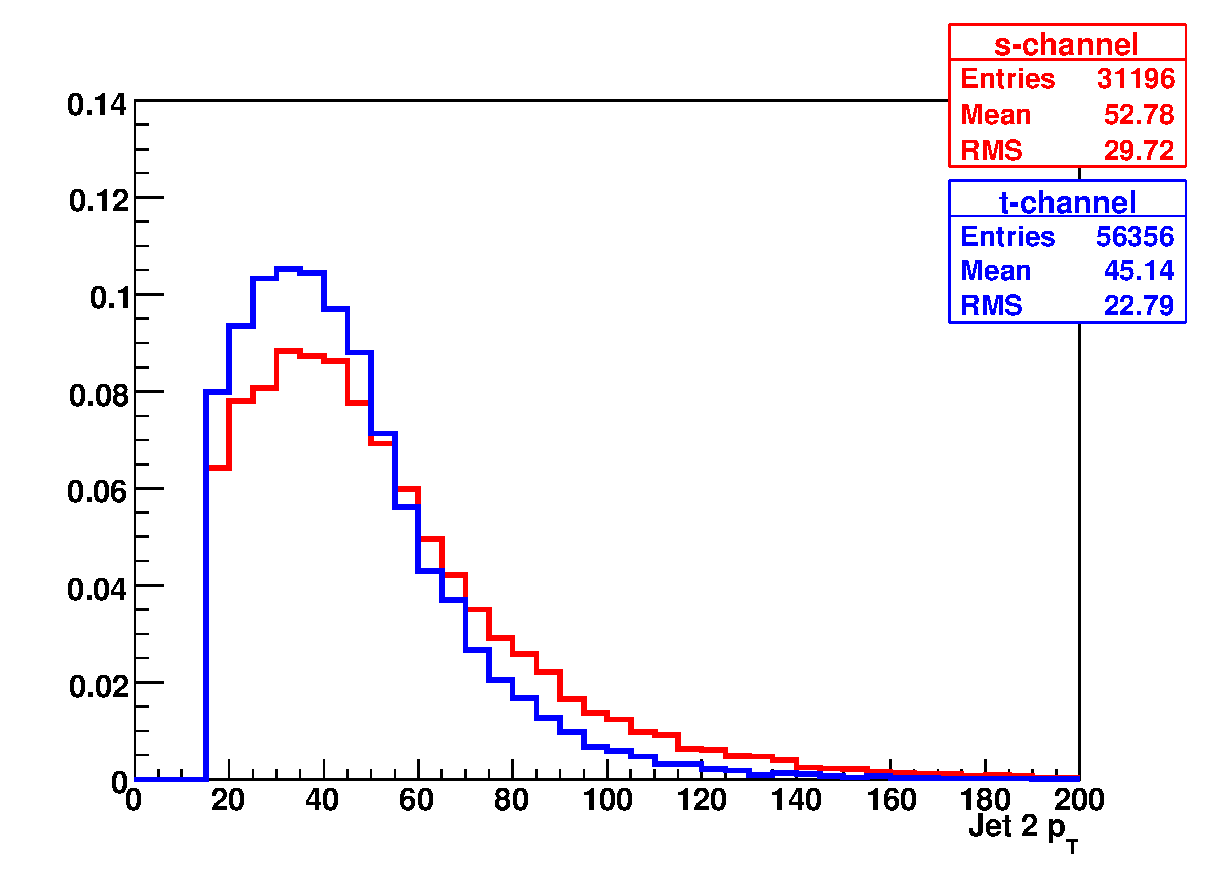
\includegraphics[width=0.48\textwidth]{eps/Analysis/Jet2Pt.eps}
\includegraphics[width=0.48\textwidth]{eps/Analysis/Jet2Eta.eps}
\end{center}
\vspace{-0.1in}
\caption{Second leading jet $p_{T}$ (left) and $\eta$ (right) distributions for $s$-channel (red) and $t$-channel (blue) single top. The second leading jet is required to have $p_{T}>20$~GeV and $|\eta|<3.4$}
\label{stjet2}
\end{figure}


\subsection{Missing $E_{T}$}
\label{missingetselection}

A large amount of missing transverse energy in an event can indicate the presence of a neutrino in the final state. All events are required to have M$E_{T} > 15$~GeV. Fig.~\ref{stmet} shows the missing $E_{T}$ distribution for $s$-channel and $t$-channel single top.

\begin{figure}[!h!tbp]
\begin{center}
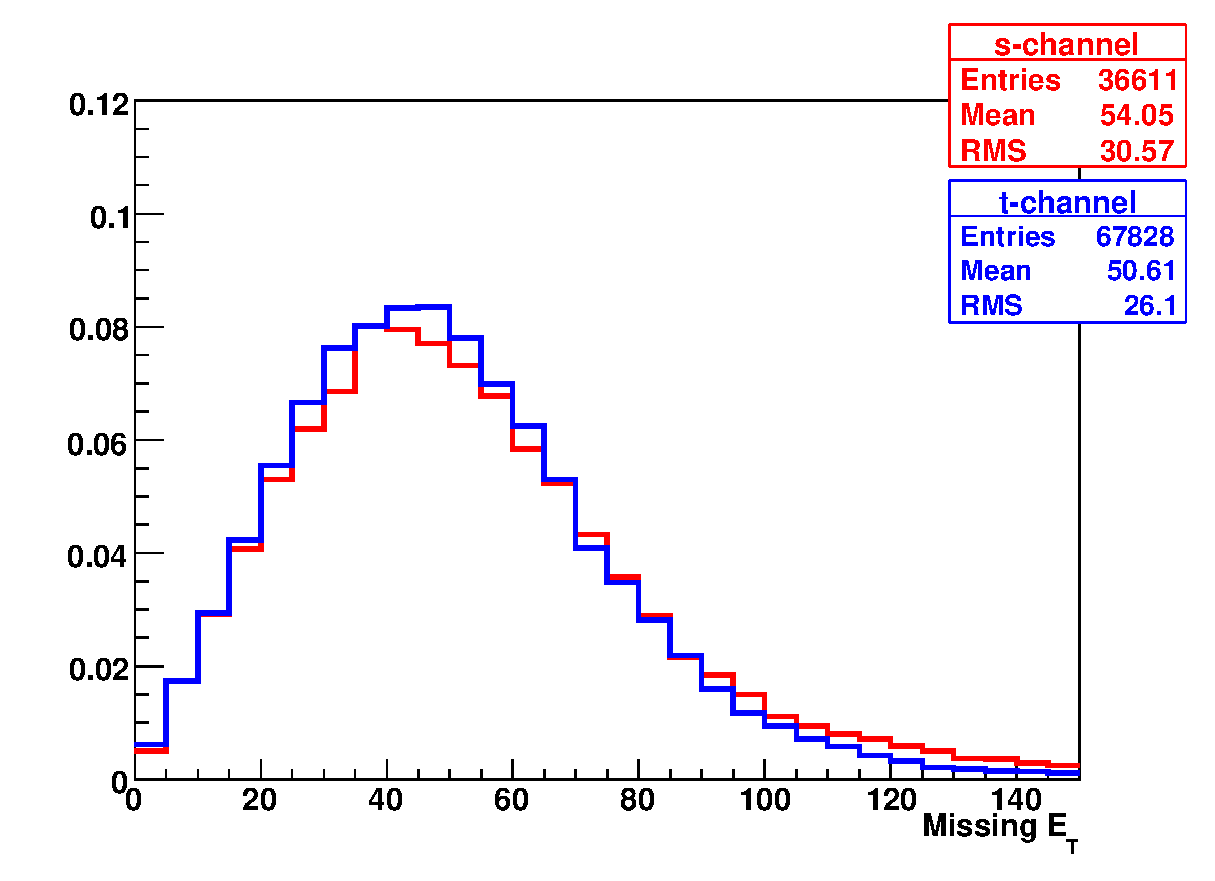
\includegraphics[width=0.48\textwidth]{eps/Analysis/MissingEt.eps}
\end{center}
\vspace{-0.1in}
\caption{Missing $E_{T}$ distribution for $s$-channel (red) and $t$-channel (blue) single top. The missing $E_{T}$ is required to larger than 15~GeV.}
\label{stmet}
\end{figure}

\subsection{Vertex Selection}
\label{vertexselection}

All events are required to have one and only one primary interaction vertex as defined in Section~\ref{pvreco}. No requirement is placed on additional minimum bias vertices in the event. Fig.~\ref{stpv} shows the primary interaction vertex longitudinal location distribution for $s$-channel and $t$-channel single top.

\begin{figure}[!h!tbp]
\begin{center}
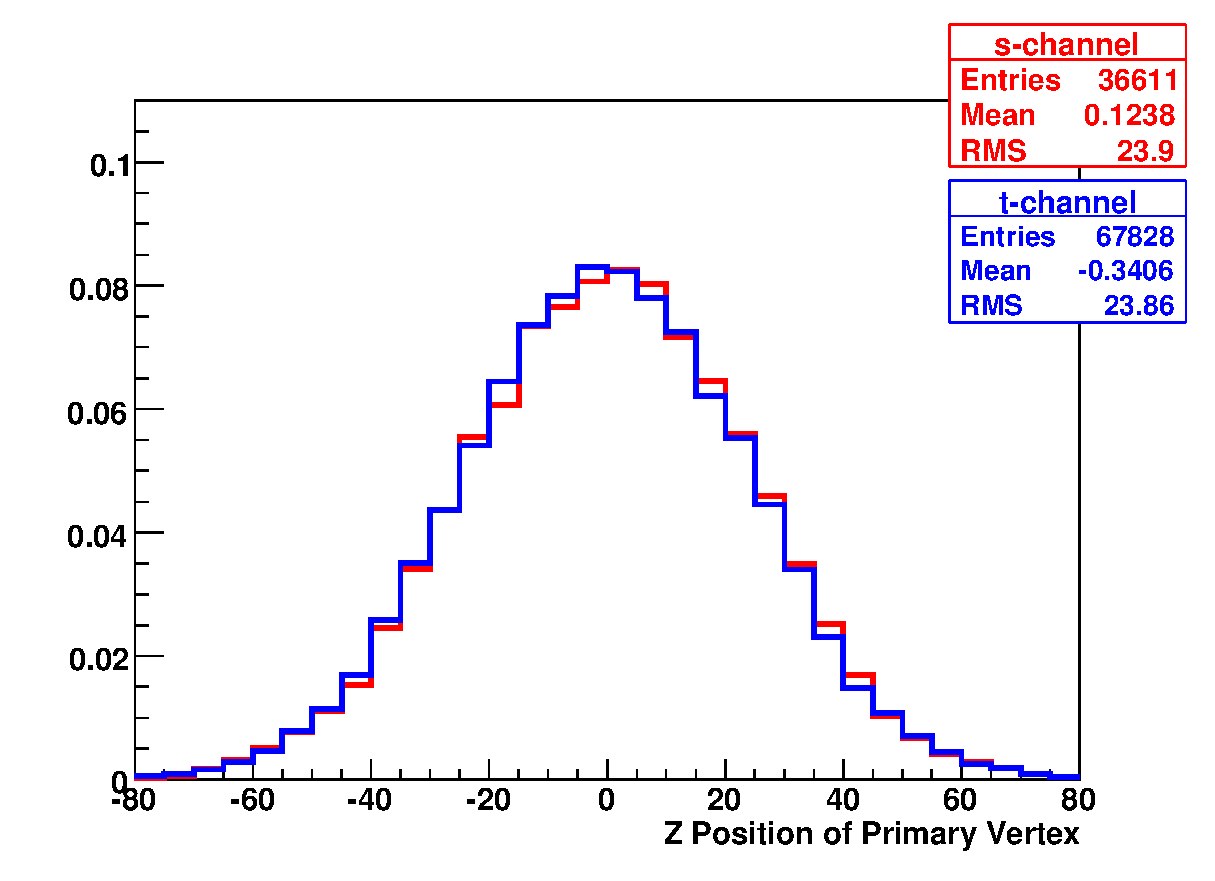
\includegraphics[width=0.48\textwidth]{eps/Analysis/PVz.eps}
\end{center}
\vspace{-0.1in}
\caption{Longitudinal location of the primary interaction vertex for $s$-channel (red) and $t$-channel (blue) single top. The primary interaction vertex is required to be located within 60~cm of the detector origin.}
\label{stpv}
\end{figure}

\subsection{b-Jet Selection}
\label{bjetselection}

Both $s$-channel and $t$-channel single top quark events have at least one b quark in the final state thus all events are required to have at least one $B$-tagged jet as identified by the neural network tagging algorithm.

\subsection{Mis-measured event rejection}
\label{misidselection}

There are several selection cuts applied to reduce mis-measured events. First, all events are required to have less than $200$~GeV of missing $E_{T}$. This cut is applied to remove events where the muon track momentum has been badly measured, which can cause a large imbalance in the missing transverse energy measurement. All events are also allowed at most three ``noise" jets. A noise jet is a jet that fails one of the criteria specified in Section~\ref{jetreco} and is not matched to an electromagnetic cluster. It has been observed that allowing more than three noise jets alters the $p_{T}$ and $\eta$~distributions of other jets in the event. The final set of cuts applied to remove unwanted events are ``triangle cuts", which are cuts between the difference in $\phi$ between an object and the missing $E_{T}$ versus the missing $E_{T}$. An example of triangle cut is shown in Fig.~\ref{triangleexample}. Three sets of triangle cuts are applied to the data and Monte Carlo events and shown in the bullets below.

\begin{itemize}
\item Electron Triangle Cuts: $|\Delta\phi(\rm{e},ME_{T})|$~vs.~$\met$
   \begin{itemize}
   \item $0<|\Delta\phi|<2$~ when $ME_{T} = 0$~GeV, and $0<ME_{T}<40$~GeV when $|\Delta\phi| = 0$
   \item $0<|\Delta\phi|<1.5$~ when $ME_{T} = 0$~GeV, and $0<ME_{T}<50$~GeV when $|\Delta\phi| = 0$
   \item  $2<|\Delta\phi|<\pi$~ when $ME_{T} = 0$~GeV, and $0<ME_{T}<24$~GeV when $|\Delta\phi| = \pi$
   \end{itemize}
\item Muon Triangle Cuts: $|\Delta\phi(\mu,ME_{T})|$~vs.~$\met$
   \begin{itemize}
   \item  $0<|\Delta\phi|<1.1$~ when $ME_{T} = 0$~GeV, and $0<ME_{T}<80$~GeV when $|\Delta\phi| = 0$
   \item  $0<|\Delta\phi|<1.5$~ when $ME_{T} = 0$~GeV, and $0<ME_{T}<50$~GeV when $|\Delta\phi| = 0$
   \item $2.5<|\Delta\phi|<\pi$~ when $ME_{T} = 0$~GeV, and $0<ME_{T}<30$~GeV when $|\Delta\phi| = \pi$
   \end{itemize}
\item Leading Jet Triangle Cut: $|\Delta\phi(\rm{Jet_{1}},ME_{T})|$~vs.~$\met$
   \begin{itemize}
   \item $1.5<|\Delta\phi|<\pi$~ when $ME_{T} = 0$~GeV, and $0<ME_{T}<35$~GeV when $|\Delta\phi| = \pi$
   \end{itemize}
\end{itemize}



\begin{figure}[!h!tbp]
\begin{center}
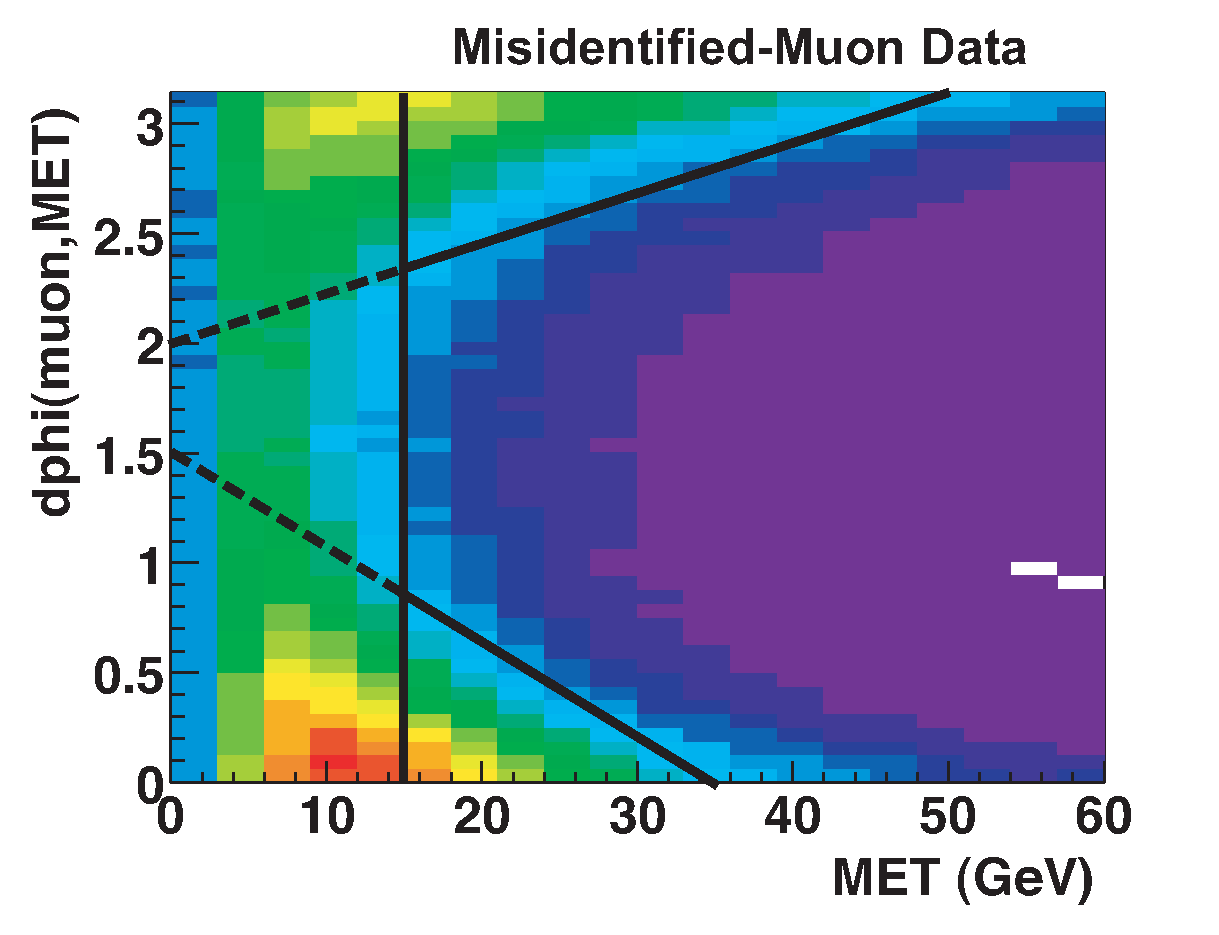
\includegraphics[width=0.48\textwidth]{eps/Reco/TriangleExample.eps}
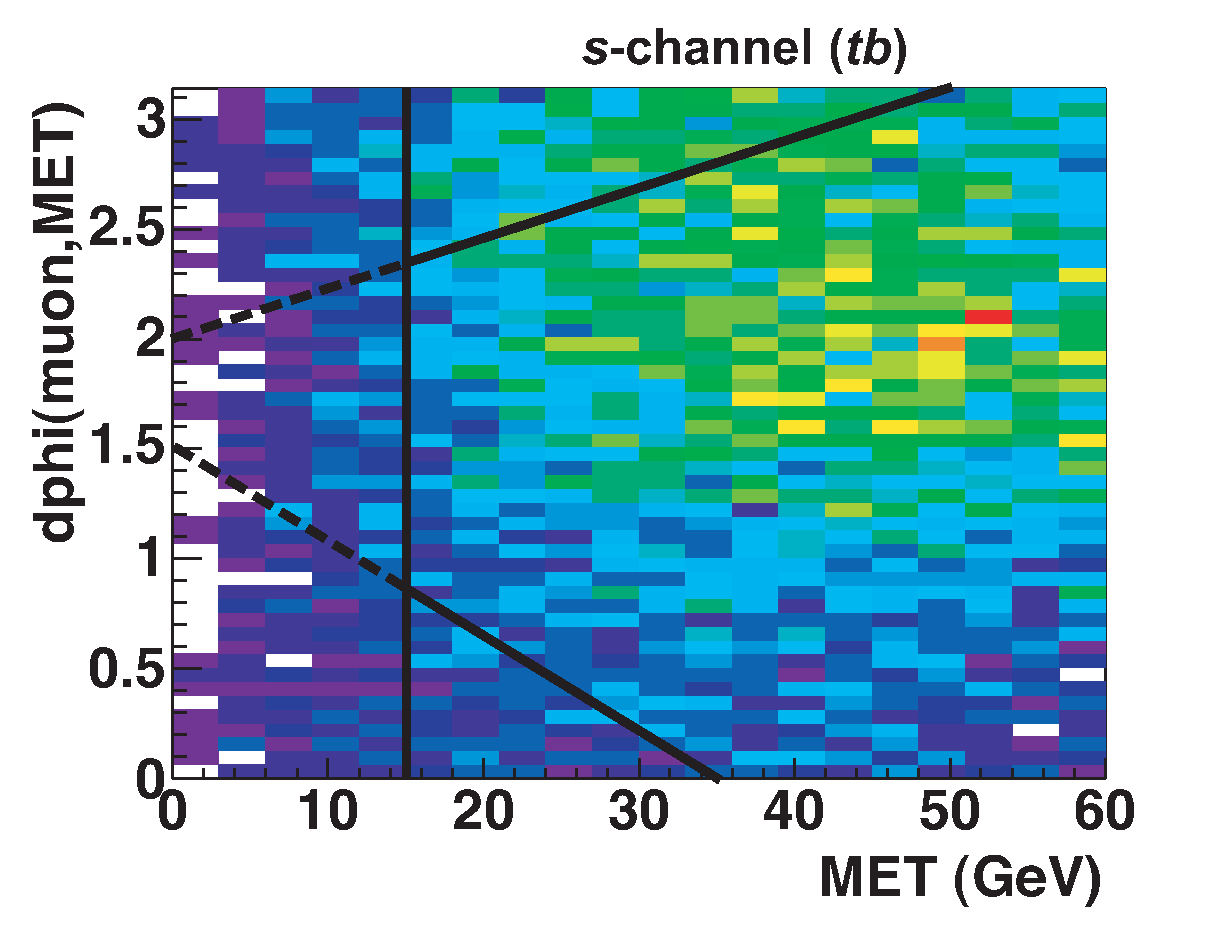
\includegraphics[width=0.48\textwidth]{eps/Reco/TriangleExampleSignal.eps}
\end{center}
\vspace{-0.1in}
\caption{Example triangle cut between a muon and the missing $E_{T}$ for mis-measured events (left) and $s$-channel single top events (right). The colors indicate the density of events. The brighter colors indicate more densely populated regions. Events which fall inside the triangles are removed from the final data sample. The black line at M$E_{T}=15$~GeV indicates the standard missing $E_{T}$ selection~\cite{oldsingletopnote}.} 
\label{triangleexample}
\end{figure}

\subsection{Acceptance for Single Top Quark Events}
\label{acceptance}

The signal acceptance is defined as:

\begin{equation}
\mathcal{A} = \frac{1}{\rm{N}_{\rm initial}}
\sum_{i}^{\rm{N}_{\rm selected}} \left[ \varepsilon_{\rm trigger} \times
\varepsilon_{\rm corrections} \times \varepsilon_{\rm TRF} \right]
\end{equation}

\noindent where $\rm{N}_{\rm initial}$ is the initial
number of events in each MC sample, $\rm{N}_{\rm selected}$ is the number of MC events
remaining after selection, $\varepsilon_{\rm{trigger}}$ is the trigger weight, $\varepsilon_{\rm{corrections}}$ are the Monte Carlo correction factors, and $\varepsilon_{\rm{TRF}}$ is the $B$-tagging weight. Table~\ref{acceptances} shows the percentage of each single top quark
signal for each jet multiplicity that remain after selection cuts.


\vspace{0.2in}
\begin{table}[!h!tbp]
\begin{center}
\caption{Single acceptances after selection cuts, one, and two $B$-tags. The branching ratio for $W\rightarrow \ell\nu$~is included in the acceptance.}
\label{acceptances}
\begin{tabular}{c|ccc|ccc}
%\multicolumn{7}{c}{\hspace{1in}\underline{$s$-channel and $t$-channel Signal Acceptances}}\vspace{0.1in} \\
& \multicolumn{3}{c|}{Electron Channel} & \multicolumn{3}{c}{Muon Channel} \\
                     & 2 jets & 3 jets & 4 jets
                     & 2 jets & 3 jets & 4 jets \\
\hline
Before $B$ tagging	&        	&        	&        	&        	&        	&        	\\
~~$tb$               		& 1.77\%	& 0.83\% 	& 0.23\%	& 1.36\% 	& 0.69\% 	& 0.19\%	\\
~~$tqb$              	& 1.49\% 	& 0.79\% 	& 0.25\% 	& 1.17\% 	& 0.64\% 	& 0.20\%	\\
\hline
One $B$-tagged jet   &        	&        	&        	&        	&        	&        	\\
~~$tb$               		& 0.82\% 	& 0.39\% 	& 0.11\% 	& 0.64\% 	& 0.32\% 	& 0.09\%	\\
~~$tqb$              	& 0.61\% 	& 0.34\% 	& 0.11\% 	& 0.50\% 	& 0.28\% 	& 0.09\%	\\
\hline
Two $B$-tagged jets	&        	&        	&        	&        	&        	&        	\\
~~$tb$               		& 0.29\% 	& 0.14\% 	& 0.04\% 	& 0.24\% 	& 0.12\% 	& 0.03\%	\\
~~$tqb$              	& 0.02\% 	& 0.05\% 	& 0.02\% 	& 0.01\% 	& 0.04\% 	& 0.02\%
\end{tabular}
\vspace{-0.1in}
\end{center}
\end{table}